\documentclass[xcolor=dvipsnames]{beamer} 
\usetheme{umbc1} 
\usepackage{textpos}
\usepackage{amsmath}
\usepackage{graphicx}
\usepackage[flushleft]{threeparttable}
\usepackage{color, colortbl}
\usepackage{multirow} 
\usepackage{booktabs,xcolor,siunitx}
\usepackage[scale=2]{ccicons}
\usepackage[framemethod=tikz]{mdframed}
\usepackage{hyperref}
\usepackage{caption}
\usepackage[ddmmyyyy]{datetime}
\usepackage{textcomp}
\usepackage{verbatim}
\usepackage{ragged2e}
\hypersetup{
colorlinks=false,     
    linkcolor=red
}
\usepackage[T1]{fontenc}


\begin{document}
\vspace{-2cm}
\title[Workshop \LaTeX{}]{\textbf{Workshop on\\``Document typesetting and Processing using \LaTeX{}''} \vspace{-0.5cm}}

\author[\today, \ccby{} P. K. Yadav \&  F. A. Faroque]{\textbf{\vspace{-0.5cm}Session: Hello \LaTeX{}}}
\institute{\href{http://www.texample.net/tikz/examples/india-map/}{
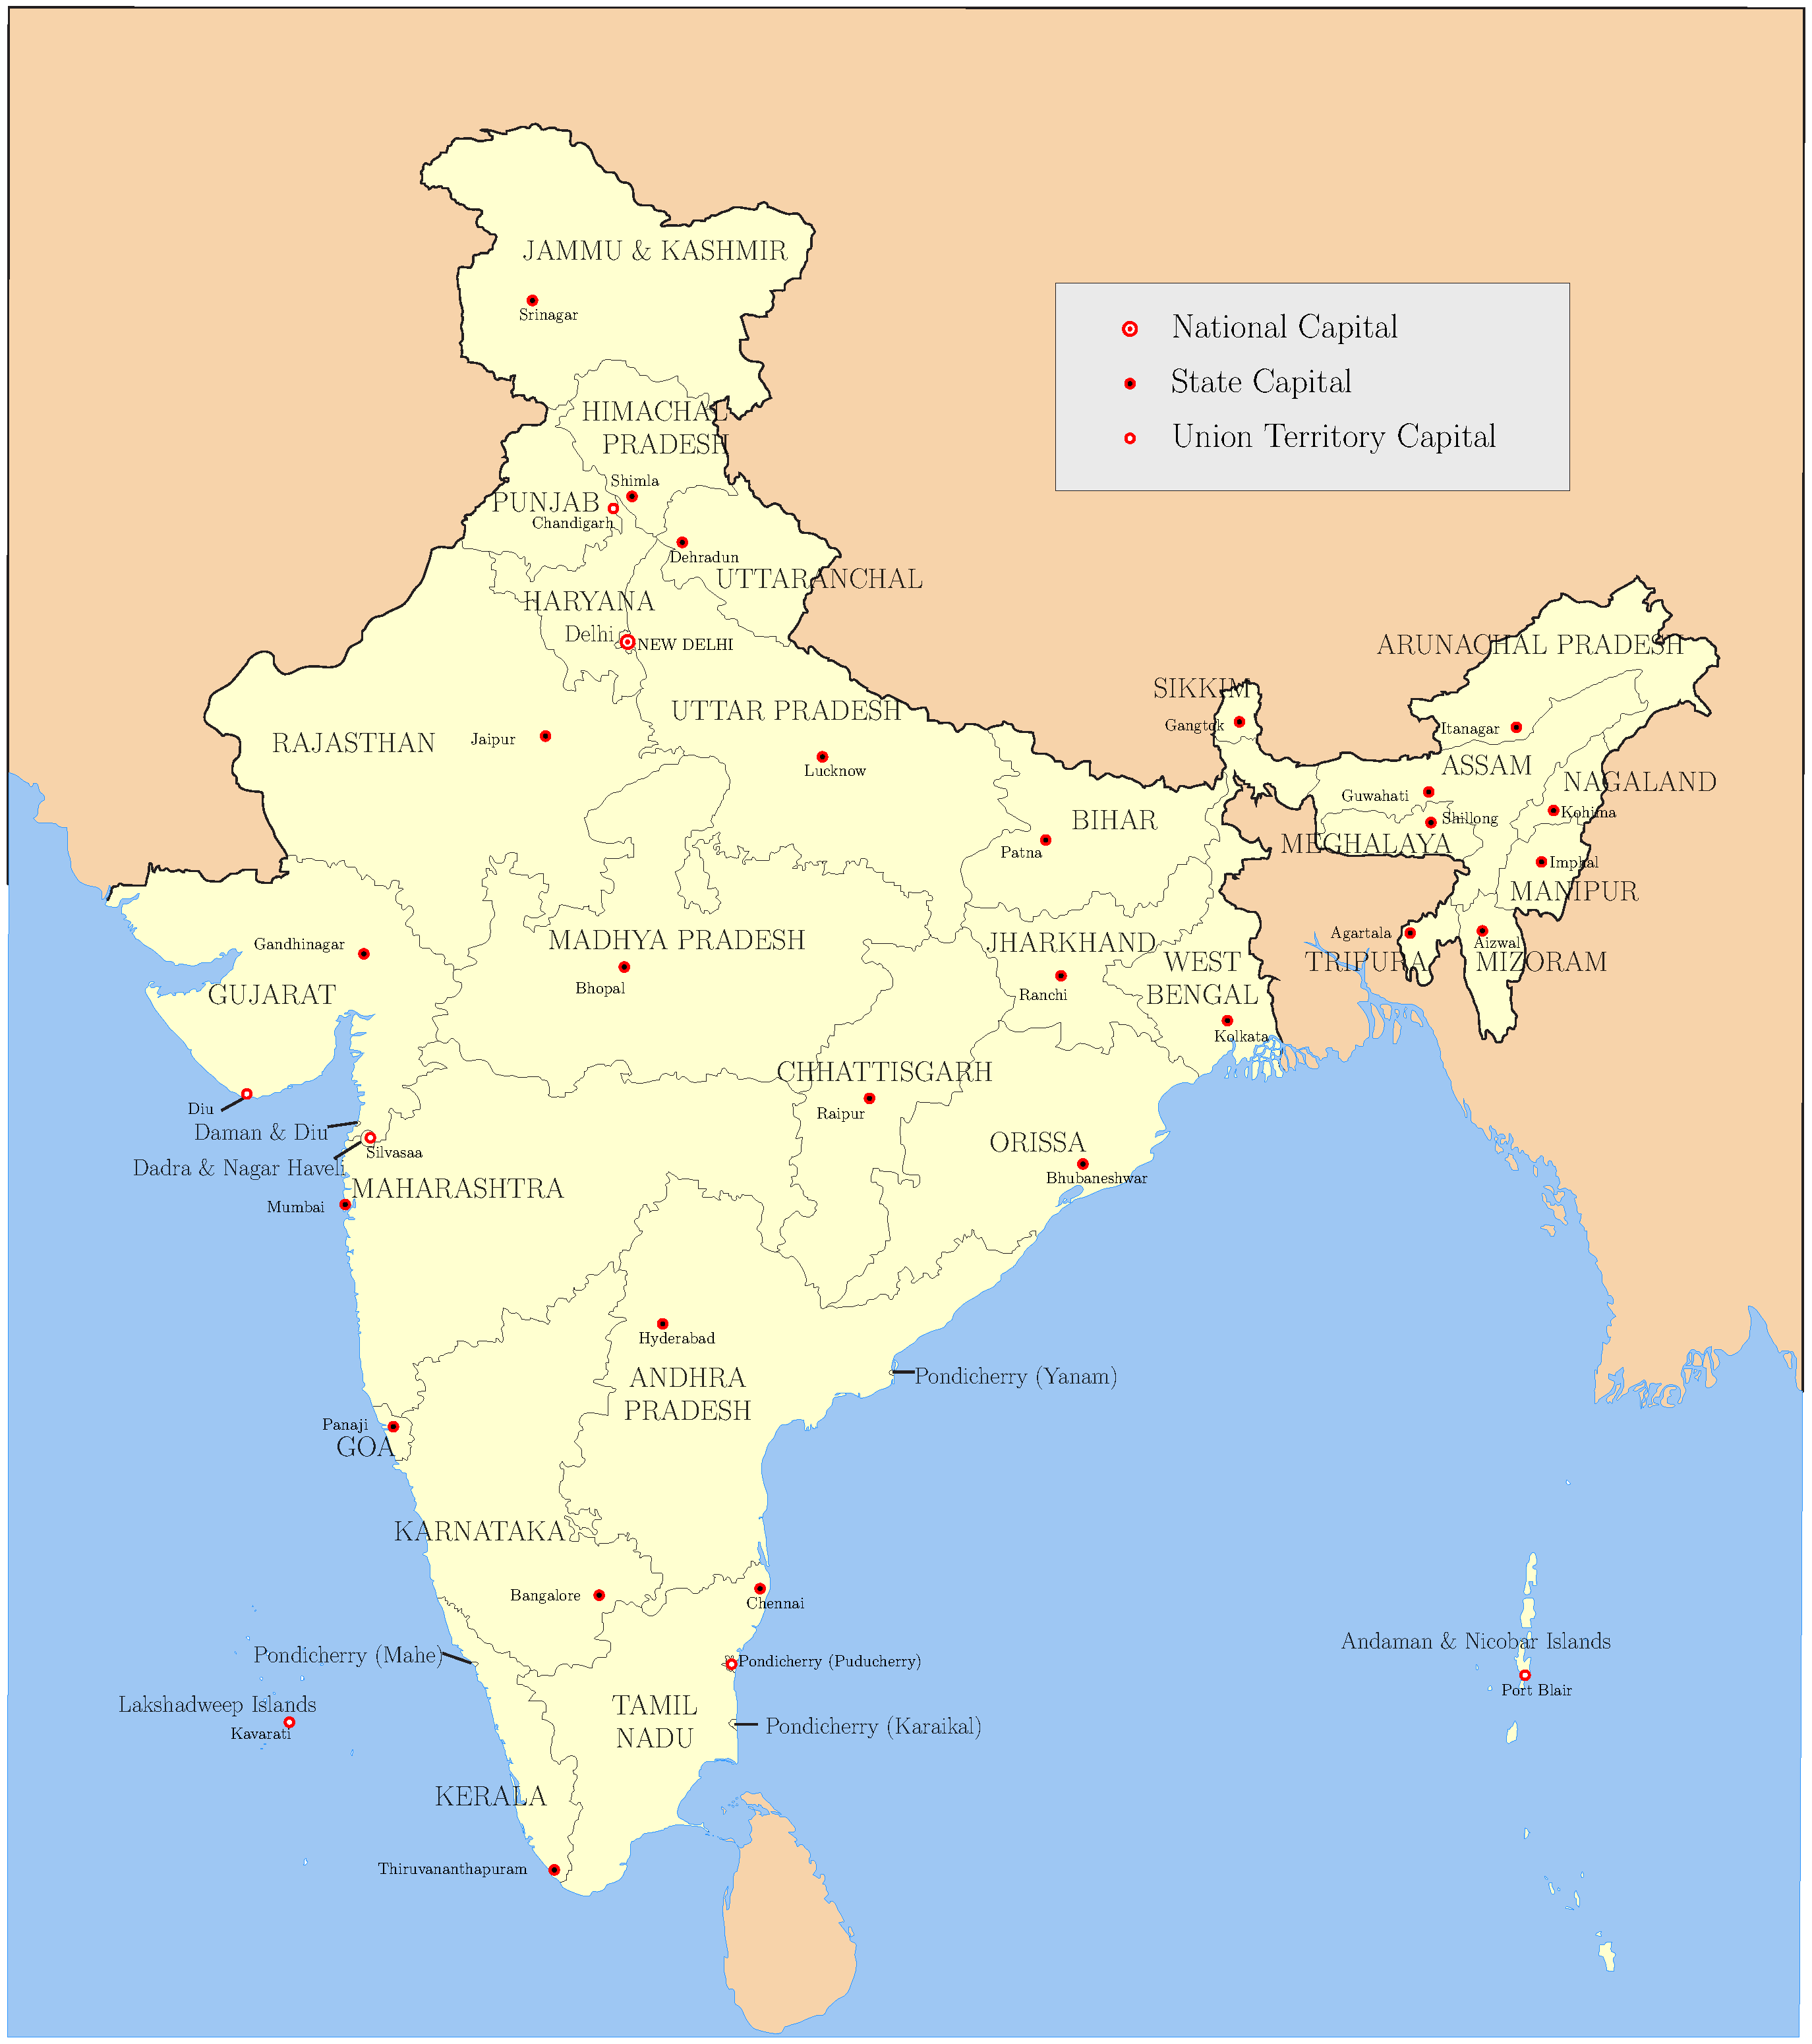
\includegraphics[scale=0.06]{fig/imap}}\centering\\
\begin{flushleft}
Presented by: \textbf{P.K. Yadav \& F. A. Faroque} \\
\hspace{1.85cm}\textbf{Department of Civil Engineering} \hspace{2.5 cm} \today
\end{flushleft}
}       

\date{}




{
\setbeamertemplate{footline}{} 
\begin{frame}
\begin{textblock*}{50cm}(0\textwidth,0cm)
%\begin{textblock*}{120mm}(.75\textwidth,-1.5cm)

\includegraphics[width=5cm]{fig/logofinal}
\end{textblock*}
\vspace{1.2cm}


  \titlepage
\end{frame}
}
\addtocounter{framenumber}{-1}
%\vskip0.4cm
\logo{
\includegraphics[width=1.2cm,height=1.2cm,keepaspectratio]{fig/mujlogo4}}

\section{Motivation}
\begin{frame}{\textbf{Motivation: Why \LaTeX{}}}
\begin{enumerate}
\item \LaTeX{} allows you to  \textbf{``clearly separate the content from the format of your document''}. \par
\vspace{0.4cm}

\justifying {This gives you the opportunity to focus on the ``what'', the creative part of your work, rather than the ``how'' is it going to look printed out in paper.}\par
\vspace{0.2cm}
\item \LaTeX{} provide  {\bf ``high typographical quality of the document''}.\par
\end{enumerate}
\vspace{0.4cm}
{\justifying Let us start with the ``Typographical quality'' of \LaTeX{}. The Format issues will clear itself by the end of the day.}

\end{frame}

\section{Typographical Quality}
\begin{frame}{\textbf{Typographical Quality I}}{Justification and hyphenation I}

\href{http://www.zinktypografie.nl/comparison.pdf}{
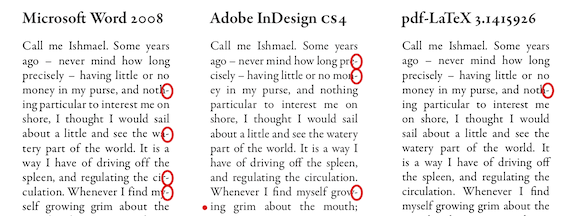
\includegraphics[scale=1.2]{fig/fig1}}\centering\\
\vspace{0.3cm}

\justifying {
\LaTeX{} uses the highly sophisticated algorithms for optimizing ``justification and hyphenation'' for an entire paragraph. \\
\vspace{0.2cm}

This results among other in irregular spacing and a high number of hyphenated words.}


\end{frame}

\begin{frame}{\textbf{Typographical Quality II}}{Justification and hyphenation II}

Statistics on word spacing in the comparison document above.

\begin{table}

\caption*{Hyphenation and inter-word spacing statistics}
\vspace{-0.6cm}
\begin{tabular}{lccc}
\toprule
& Word 2007 & InDesign & \LaTeX\\
\hline
Number of hyphenations & 9 & 10& 4\\
SD of IWS (pt) & 2.26 & 1.94 & 1.42\\
Maximum IWS (pt) & 14.4 & 13.2 & 9.0\\
Number of lines with IWS $>$ 9pt & 5 & 2 & 0\\
\bottomrule
{\tiny SD = Standard Deviation, IWS= Inter Word Spacing } 
\end{tabular}

\end{table}

\end{frame}


\begin{frame}{\textbf{Typographical Quality III}}{Ligatures}

\justifying {Some letters clash with one another if they are printed next to each other. Familiar examples are the combinations `fl' and `fi', in which the `f' touches the dot of the `i' or the top of the `l'.}\\
\vspace{0.5cm}

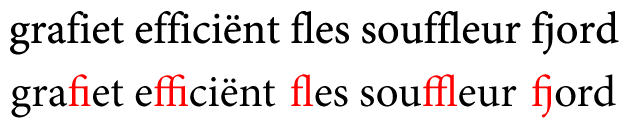
\includegraphics[scale=0.5]{fig/fig3}\centering\\
\vspace{0.2cm}

\justifying {
MS Word (top) does not automatically use ligatures. \LaTeX{} (bottom) automatically uses all supported ligatures.
}

\end{frame}

\begin{frame}{\textbf{Typographical Quality IV}}{Real smallcaps}
\justifying{
For titles, headers and abbreviations one often uses smallcaps: capitals that are just as high as normal lowercase letters.}\\
\vspace{0.5cm}

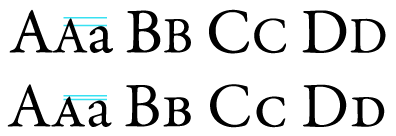
\includegraphics[scale=0.5]{fig/fig4}\centering\\
\vspace{0.4cm}


\justifying{
MS Word (top) uses scaled capitals instead of real smallcaps. \LaTeX{} (bottom) uses the real smallcaps provided in the typeface.}


\end{frame}

\begin{frame}{\textbf{Typographical Quality V}}{Kerning}
\justifying{
Kerning is placing letters closer together or further apart if the form of the letters necessitates it. This results in a much more balanced spacing, enhancing readability.}\\
\vspace{0.5cm}

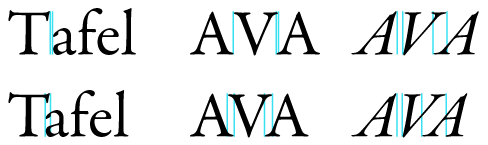
\includegraphics[scale=0.5]{fig/fig5}\centering\\
\vspace{0.2cm}

\justifying{
MS Word (top) uses the wrong, average kerning for the letter pairs `Ta', `AV' and `VA'. \LaTeX{} (below) uses the right kerning as prescribed in the font's kerning tables.
}

\end{frame}

\begin{frame}{\textbf{Typographical Quality VI}}{Mathematical Writing}

Compare by yourself:


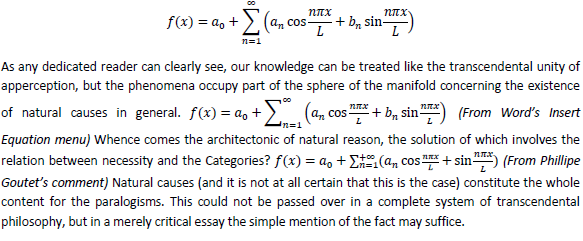
\includegraphics[scale=0.5]{fig/fig6}\centering\\
\vspace{0.2cm}

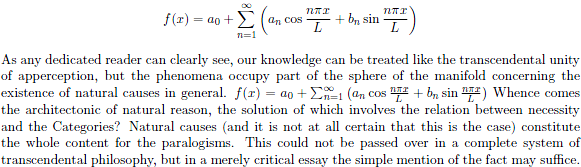
\includegraphics[scale=0.5]{fig/fig7}\centering\\
\vspace{0.2cm}
\justifying{
MS Word (top) and \LaTeX{} (below) uses the right kerning as prescribed in the font's kerning tables.
}

\end{frame}

\section{Other Advantage of \LaTeX}
\begin{frame}{\textbf{Other Advantage of \LaTeX{} over Word Processors}}
\setbeamercovered{transparent}
\begin{enumerate}[<+->]
\item The consistency of the layout
\vspace{0.2cm}
\item Easily produce PDFs with hyperlinks, table of contents, indices, etc.
\vspace{0.2cm}
\item Guaranteed backward compatibility (Word 2007 and 2013 have different format)
\vspace{0.2cm}
\item The excellent referencing system
\vspace{0.2cm}
\item Extremely customizable
\vspace{0.2cm}
\item Free of cost
\vspace{0.2cm}
\end{enumerate}
\end{frame}

\section{Disadvantage of \LaTeX}
\begin{frame}[fragile]{\textbf{Disadvantage of \LaTeX{} I}}
\begin{enumerate} \item A very steep learning curve. Our first slide was coded as:
\end{enumerate}
\vspace{-0.5cm}
\small \color{gray!80!blue}
\begin{verbatim}
 \begin{frame}[fragile]{Motivation: Why \LaTeX{}}
 \begin{enumerate}
\item \LaTeX{} allows you to \textbf{``clearly separate
  the content from the format of your document"}. \par
 \vspace{0.2cm}
 
 This gives you the opportunity to focus on the ``what", 
 the creative part of your work, rather than the ``how" 
 is it going to look printed out in paper.\par
 \vspace{0.2cm}
 \item \LaTeX{} provide  {\bf ``high typographical 
 quality of the documents"}.\par
 \end{enumerate}
\end{verbatim}
 \verb|\end{frame}|
%\end{verbatim}


\end{frame}

\begin{frame}[fragile]{\textbf{Disadvantage of \LaTeX{} II}}
\setbeamercovered{transparent}
\begin{enumerate}[<+->]\setcounter{enumi}{1}
 
\item Distributed information on modules
\vspace{0.2cm}
\item Absence of collaborative editing
\vspace{0.2cm}
\item Grammatical check is missing
\vspace{0.2cm}
\item Layout changes are difficult
\item Adding picture and table is relatively difficult compared to MS Word, although better output is obtained. \\

\end{enumerate}
\pause
\vspace{0.2cm}
Now that we have decided to use \LaTeX{}, let us get started with first, with the word TEX.

\end{frame}

\section{Introducing \LaTeX{}}
\begin{frame}{\textbf{The \LaTeX{} History}}
\begin{columns}

\column{.2\textwidth}
\href{http://en.wikipedia.org/wiki/Donald_Knuth}{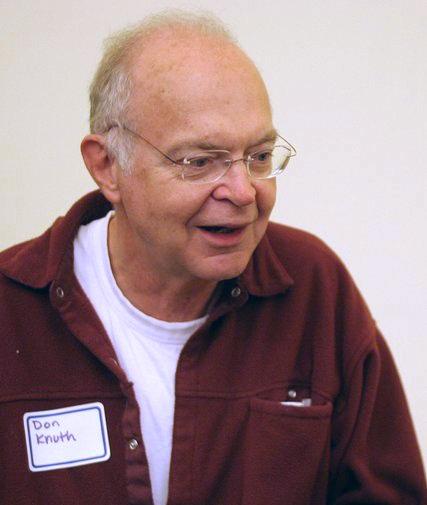
\includegraphics[scale =0.2]{fig/fig8}}\\
\vspace{-0.3cm}
\hspace{0.3cm}\textit{\tiny Donald E. Knuth}
\vfill
\column{.8\textwidth}
\justifying{ \TeX(= tau epsilon chi, and pronounced similar to `tech') is a computer language designed by Donald E. Knuth of Stanford University. The first version of \TeX{} was released in 1978 and the current version is 3.1415926 (absolutely bug free that the version is converging to the value of $\pi$) }\\

\end{columns}
\vspace{0.5cm}
\textcolor{red}{Then what is \LaTeX{}?}\\

\begin{columns}

\column{.2\textwidth}
\vspace{0.5cm}
\href{http://en.wikipedia.org/wiki/Leslie_Lamport}{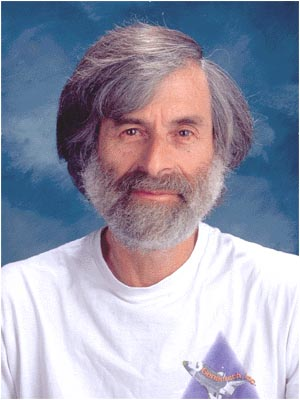
\includegraphics[scale =0.2]{fig/fig9}}\\
\vspace{-0.3cm}
\hspace{0.3cm}\textit{\tiny Leslie Lamport}
\vfill

\column{.8\textwidth}

\justifying{\LaTeX{} is a document preparation based on the \TeX{}  formatter developed by Leslie Lamport. This system adds a set of functions that makes the  language more friendlier than using the primitives provided in \TeX. Thus, we use \LaTeX{} and not \TeX}

\end{columns}

\end{frame}

\section{Getting Started with \LaTeX{}}
\begin{frame}{\textbf{Getting Started with \LaTeX{}}}

\justifying {That we know \LaTeX{} is rather a coding, let us find that we need to run our code. The figure below will illustrate.}\\
\vspace{0.5cm}
\begin{columns}
\column{0.7\textwidth}
\vfill
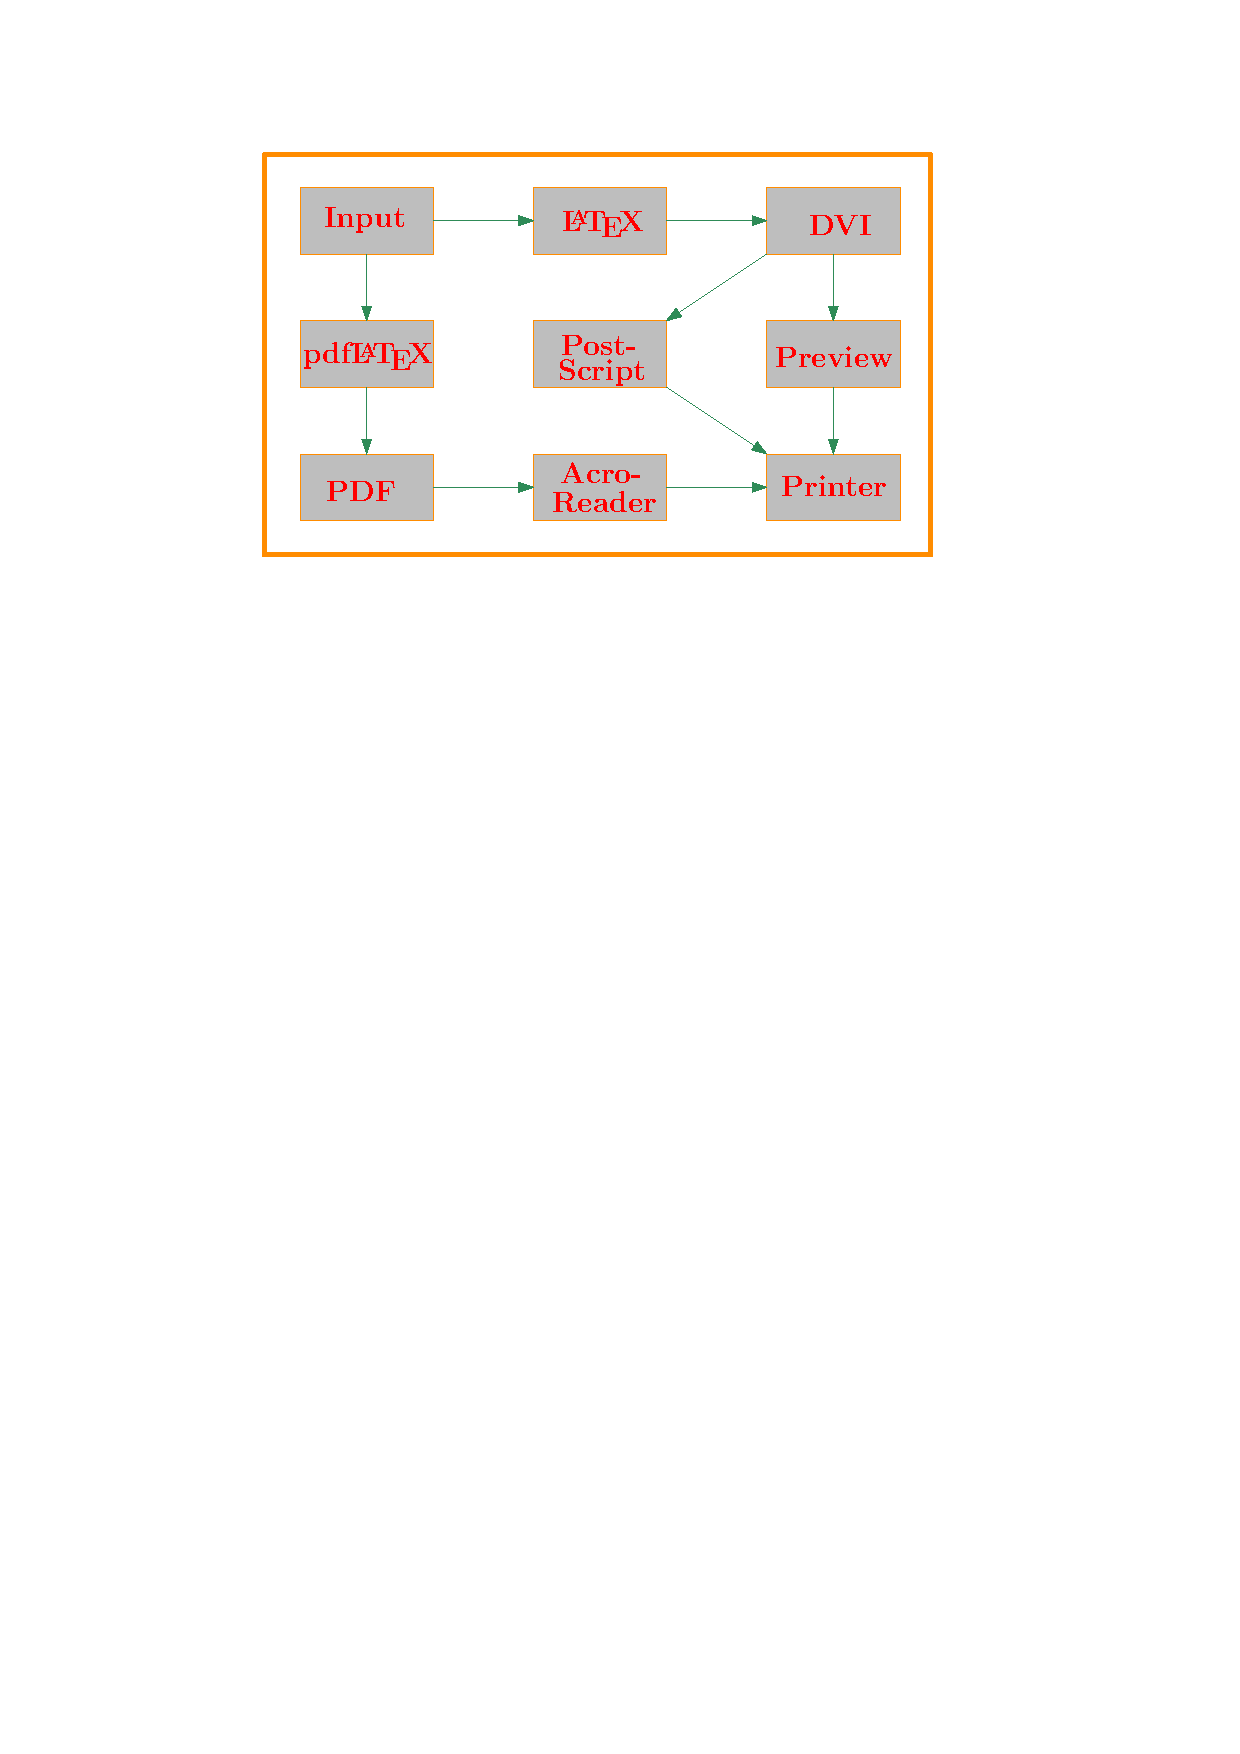
\includegraphics[scale =0.5]{fig/fig10}\centering
\column{0.5\textwidth}

We require:\\

\begin{enumerate}

\item An input system: A text editor, we will use \textbf{TeXstudio }
\item A \LaTeX processor
\item A PDF reader

\end{enumerate}


\end{columns}
\vspace{0.8cm}
\textbf{Next, we install a \LaTeX{} system.}

\end{frame}
{
\setbeamertemplate{footline}{} 
\begin{frame}{\Huge \textbf{Installing$\ldots$,}}
\pagestyle{plain}
\Huge

\textbf{Next, your first \LaTeX{} document.}


\end{frame}

}

\end{document}
